\chapter{Laster}
I det følgende afsnit vil de laster der påvirker tilbygningen til Strøybergs Palæ. Lasterne der påvirker konstruktionen er nytte-, egen-, vind- og snelast. Lasterne skal være kendt, før bygningen og fundamentet kan dimensioneres.

\section{Nyttelast}
Nyttelast er en last der ikke virker permanent på en bygning, men derimod er varierende og kommer af anvendelse af en bygning. Nyttelast er den last som mennesker og inventar påvirker en konstruktion med. Nyttelast dækker over to laster, den transiente del (laster der varer over en til tre dage) og den vedvarende del (laster der varer over fem til ti år).

Nyttelast regnes på to forskellige måder, en jævnt fordelt fladelast $ q_{k} $ målt i $ \SI{}{kN/m^2} $ og en punktlast $ Q_{k} $, målt i kN. Disse to nyttelaster kan ikke optræde samtidigt. Fladelasten bruges til en global eftervisning af bæreevne og punktlasten bruges til en lokaleftervisning af bæreevne.


Nyttelasten, der virker på tilbygningen, er ens på alle etager. Bygningen er beregnet til boliger og går derfor ind under kategori A, som beskrevet i den tilhørende Eurocode. I kategori A regnes der med en anbefalet karakteristisk jævnt fordelt nyttelast på $\SI{2}{kN/m^2}$ og en punktlast på $\SI{2}{kN/m^2}$


\newpage

\section{Egenlast}
	Egenlasten er udregnet ud fra 3D modeller, så materialeforbruget fremgår klart og tydeligt. Egenlasten indebærer ydervæggene, etageadskillelse, taget og naturligvis stålskelettet.
	
	Eftersom der regnes på en ramme ved siden af midten af hele bygningen, ser rammen således ud
\begin{figure}[H] 
	\centering
	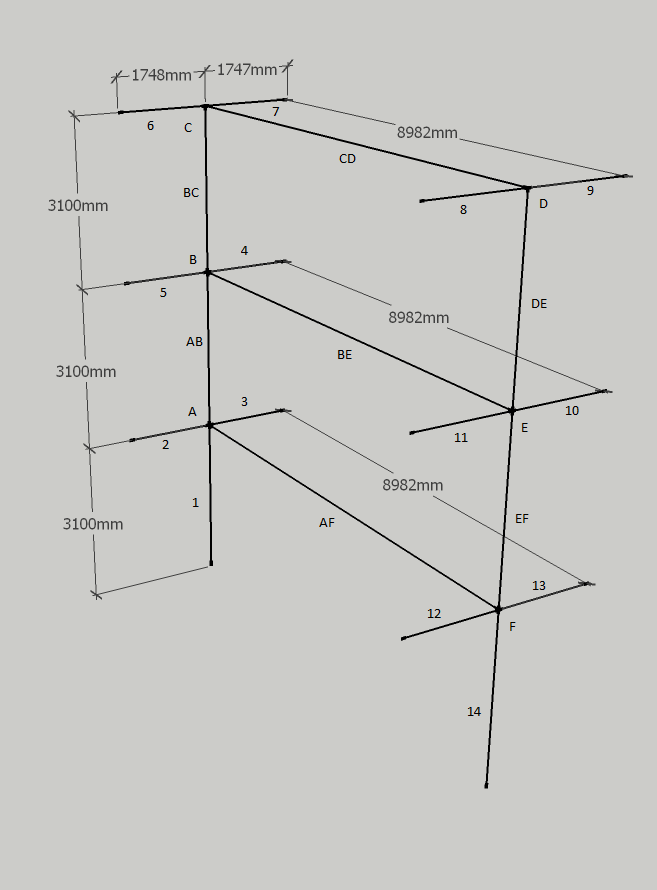
\includegraphics[width=0.7\textwidth]{billeder/Staaldimensioner_5}
	\caption{Viser en 3D model af rammens stållayout }
	\label{fig:EL1}
\end{figure}	
	\newpage
	Denne ramme bærer altså denne mængde af bygningen
\begin{figure}[H] 
	\centering
	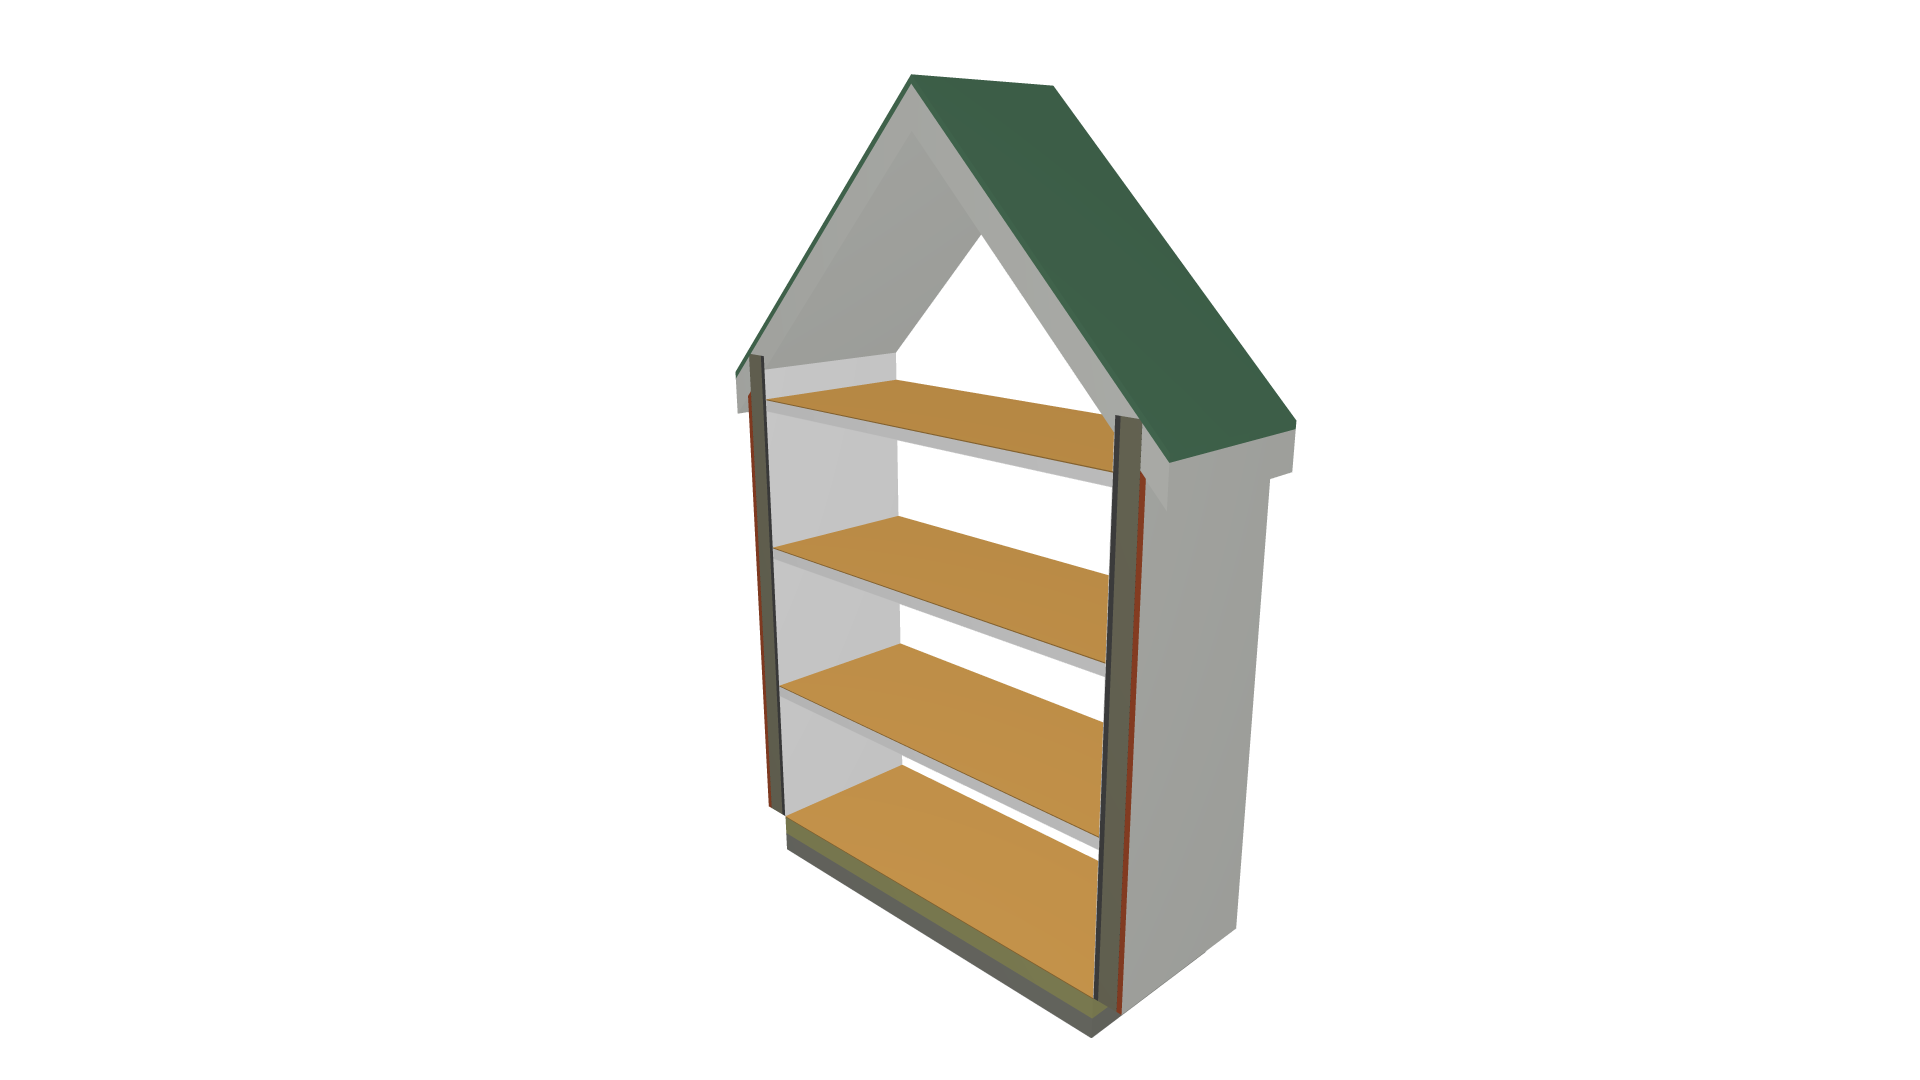
\includegraphics[width=1\textwidth]{billeder/Tvaersnit1}
	\caption{Viser en 3D model af de elementer, som stålrammen på Figur \ref{fig:EL1} bærer}
	\label{fig:EL2}
\end{figure}

I tabellen herunder ses ydervæggenes opbygning. Tallene er for den ene side af bygningen, altså det som halvdelen af rammen bærer.
\begin{table}[H]
	\centering
	\begin{tabular}{lll|l|ll|l|l}
		\cline{4-4} \cline{7-7}
		&                                                        &      & Mængde ($m^{3}$) &                             &      & Vægt (kg) &                             \\ \hline
		\multicolumn{1}{|l|}{}           & \multicolumn{1}{l|}{Densitet ($\dfrac{kg}{m^{3}}$)} & St.  & 1. sal                       & \multicolumn{1}{l|}{2. sal} & St.  & 1. sal    & \multicolumn{1}{l|}{2. sal} \\ \hline
		\multicolumn{1}{|l|}{Teglsten}   & \multicolumn{1}{l|}{1500}                              & 1,17 & 1,17                         & \multicolumn{1}{l|}{1,17}   & 1755 & 1755      & \multicolumn{1}{l|}{1755}   \\ \hline
		\multicolumn{1}{|l|}{Mineraluld} & \multicolumn{1}{l|}{115}                               & 4,33 & 4,33                         & \multicolumn{1}{l|}{4,33}   & 498  & 498       & \multicolumn{1}{l|}{498}    \\ \hline
		\multicolumn{1}{|l|}{Gips}       & \multicolumn{1}{l|}{900}                               & 0,13 & 0,13                         & \multicolumn{1}{l|}{0,13}   & 117  & 117       & \multicolumn{1}{l|}{117}    \\ \hline
		\multicolumn{1}{|l|}{SUM}        & \multicolumn{1}{l|}{}                                  & 5,63 & 5,63                         & \multicolumn{1}{l|}{5,63}   & 2371 & 2371      & \multicolumn{1}{l|}{2371}   \\ \hline
	\end{tabular}
	\caption{Viser densitet af de anvendte materialer, samt materialeforbruget og massen på de forskellige etager}
	\label{tabel:EL1}
\end{table}

I tabellen herunder ses gulvenes opbygning. Tallene er for den ene side af bygning, altså det som halvdelen af rammen bærer.
\begin{table}[H]
	\centering
	\begin{tabular}{lll|l|ll|l|l}
		\cline{4-4} \cline{7-7}
		&                                                        &       & Mængder ($ m^{3} $) &                            &      & Vægt (kg) &                             \\ \hline
		\multicolumn{1}{|l|}{}          & \multicolumn{1}{l|}{Densitet ($ \dfrac{kg}{m^{3}} $)} & St.   & 1. sal                        & \multicolumn{1}{l|}{2.sal} & St.  & 1. sal    & \multicolumn{1}{l|}{2. sal} \\ \hline
		\multicolumn{1}{|l|}{Træ}       & \multicolumn{1}{l|}{500}                               & 0,314 & 0,314                         & \multicolumn{1}{l|}{0,314} & 157  & 157       & \multicolumn{1}{l|}{157}    \\ \hline
		\multicolumn{1}{|l|}{Hul beton} & \multicolumn{1}{l|}{2000}                              & 3,45  & 3,45                          & \multicolumn{1}{l|}{3,45}  & 6906 & 6906      & \multicolumn{1}{l|}{6906}   \\ \hline
		\multicolumn{1}{|l|}{Gips}      & \multicolumn{1}{l|}{900}                               & 0,157 & 0,157                         & \multicolumn{1}{l|}{0,157} & 141  & 141       & \multicolumn{1}{l|}{141}    \\ \hline
		\multicolumn{1}{|l|}{SUM}       & \multicolumn{1}{l|}{}                                  & 3,92  & 3,92                          & \multicolumn{1}{l|}{3,92}  & 7204 & 7204      & \multicolumn{1}{l|}{7204}   \\ \hline
	\end{tabular}
	\caption{Viser densitet af de anvedte materialer, samt materialeforbruget og massen på de forskellige etager}
	\label{tabel:EL2}
\end{table}

\newpage
I tabellen herunder ses tagets opbygning. Tallene er for den ene side af taget, altså det som halvdelen af rammen bærer.
\begin{table}[H]
	\centering
	\begin{tabular}{l|l|l|l|}
		\cline{2-4}
		& Densitet ($ \dfrac{kg}{m^{3}} $) & Mængde ($ m^{3} $) & Vægt (kg) \\ \hline
		\multicolumn{1}{|l|}{Tagsten}    & 2000                              & 0,522                        & 1044      \\ \hline
		\multicolumn{1}{|l|}{Mineraluld} & 115                               & 26,1                         & 3003      \\ \hline
		\multicolumn{1}{|l|}{SUM}        &                                   & 26,6                         & 4047      \\ \hline
	\end{tabular}
	\caption{Viser densitet af de anvedte materialer, samt materialeforbruget og massen af taget}
	\label{tabel:EL3}
\end{table}

Eftersom det i udregningen af egenlasten ikke vides, hvilke stålprofiler der skal benyttes, bliver disse indsat som konstanter i udregningerne, hvorved man efterfølgende i styrkeberegningerne kan finde frem til hvilke typer, der er passende.

\begin{figure}[H] 
	\centering
	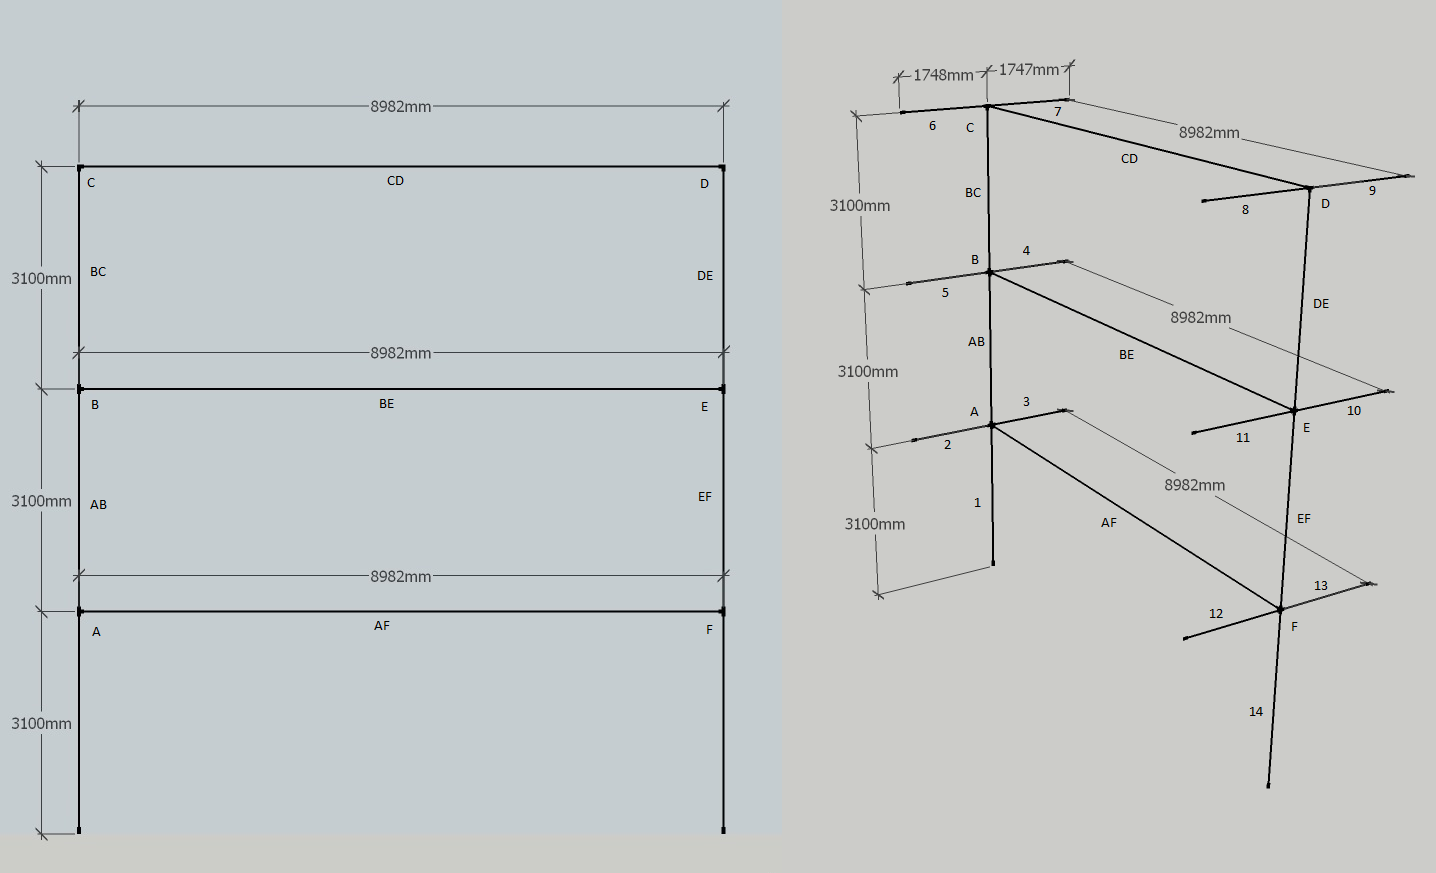
\includegraphics[width=1\textwidth]{billeder/Staaldimensioner_6}
	\caption{Viser en 3D model af stålrammen samt et tværsnitlayout}
	\label{fig:EL3}
\end{figure}

Beregnigner for egenlast i punkterne C og D. Konstruktionen er som nævnt symmetrisk omkring midten, så egenlasten bliver den samme i de to punkter. Denne tendens forsætter i de resterende punkter.
\newline
Tyngdeaccelerationen, g, sættes til $ 9,82\dfrac{N}{kg} $
\newline
Massen pr. meter for stålprofilerne betegnes, G, og måles i $ \dfrac{kg}{m} $. Størrelserne varierer og er ukendte. Så en stålbjælke eller søjle skrives eksempelvis som $ G_{CD} $.
\newline
Massen af taget, som den ene side af stålrammen bærer, angives som  $ m_{tag} $. Taget er ikke lavet af stål og kan derfor ikke ses på Figur \ref{fig:EL3}, men derimod på Figur \ref{fig:EL2}
\newline
Massen af gulvene, som den ene side af stålrammen bærer, angives som $ m_{gulv_{x}} $. Så et gulv der eksempelvis bæres af bjælken CD skrives $ m_{gulv_{CD}} $
\newline
\begin{center}
	$ P_{C/D}=m_{tag}\cdot g+G_{CD}\cdot g\cdot \dfrac{1}{2}\cdot 8,982m+m_{gulv_{CD}}\cdot g =110,5kN+k$
\end{center}

Beregninger for egenlast i punkterne B og E. 
\newline
Massen af murene angives som $ m_{mur_{x}} $. Så en mur der eksempelvis bæres af søjlen BC skrives $ m_{mur_{BC}} $.
\begin{center}
	$ P_{B/E}=P_{C/D}+G_{BE}\cdot g\cdot \dfrac{1}{2}\cdot 8,982m+m_{gulv_{BE}}\cdot g+m_{mur_{BC}}\cdot g+G_{BC}\cdot g\cdot 3,100m=204,5kN+k$
\end{center}

Beregninger for egenlast i punkterne A og F
\begin{center}
	$ P_{A/F}=P_{B/E}+G_{AF}\cdot g\cdot \dfrac{1}{2}\cdot 8,982m+m_{gulv_{AF}}\cdot g+m_{mur_{AB}}\cdot g+G_{AB}\cdot g\cdot 3,100m =298,5kN+k$
\end{center}

Beregninger for egenlasten i reaktionerne $ R_{1} $ og $ R_{2} $
\begin{center}
	$ P_{R_{1}/R_{2}}=P_{A/F}+m_{mur_{1/14}}\cdot g+G_{1}\cdot g\cdot \dfrac{1}{2}\cdot 3,100m=321,8kN+k$
\end{center}






\section{Vindlast}
Vindlast er den last som vind påvirker bygninger med og virker vinkelret på bygningers overflader. 

NOTE: evt. figur der viser hvordan vind virker på en konstruktion:

Følgende afsnit er beregnet ud fra Eurocode DS/EN-1991-1-4. Værdierne for diverse konstanter og variable er aflæst i det tilhørende danske nationale anneks.

I de følgende afsnit bliver basisvindhastigheden, ruhedesfaktoren, middelvindhastigheden, turbolensintensiteten, peakhastighedstrykket og vindtrykket på tilbygningen beregnet.








\subsection{Basisvindhastighed}
Basisvindhastigheden er afhængig af retningsfaktoren, årstidsfaktoren og grundværdien for basisvindhastigheden.

Følgende formel bruges til at beregne basisvindhastigheden:
\begin{align*}
v_{b} = c_{dir} \cdot c_{season} \cdot v_{b,0}
\end{align*}

Hvor:
\begin{itemize}
\item $v_{b}$ = basisvindhastigheden.
\item $v_{b,0}$ = grundværdien for basisvindhastigheden.
\item $ c_{season} $ = årstidsfaktoren.
\item $ c_{dir} $ = retningsfaktoren.
\end{itemize}
I dette tilfælde er $ v_{b,0} $ $ \SI{24}{m/s} $, $ c_{season} $ er 1,0, da bygningen står året rundt og $ c_{dir} $ sættes til 1,0, da dette er den anbefalede værdi.

\begin{align*}
v_{b} = 1,0 \cdot 1,0 \cdot \SI{24}{m/s}
\end{align*}

Dvs. basisvindhastigheden ved tilbygningen til Strøybergs Palæ er $ \SI{24}{m/s} $.








\subsection{Ruhedsfaktor}
Ruhedsfaktoren er afhængig af ruhedslængden, terrænfaktoren og bygningens højde over terræn.

Følgende formler bruges til at beregne ruhedsfaktoren
\begin{align*}
c_{r}(z) = k_{r} \cdot ln\left(\frac{z}{z_{0}}\right)
\end{align*}
\begin{align*}
k_{r} = 0,19 \cdot ln\left(\frac{z_{0}}{z_{0,II}}\right)^{0,07}
\end{align*}

Hvor:
\begin{itemize}
\item $ c_{r}(z) $ = ruhedsfaktoren i højden z.
\item $ k_{r} $ = terrænfaktoren.
\item z = bygningens højde over terræn.
\item $ z_{0} $ = ruhedslængden.
\item $ z_{0,II} $ =0,05m, som aflæst i Tabel XX
\end{itemize}

I dette tilfælde er z = 14.85 m, $ z_{0} $ er 0,3 m, grundet terrænkategori III er valgt.


Terrænfaktoren beregnes:
\begin{align*}
k_{r} = 0,19 \cdot ln\left(\frac{\SI{0,3}{m}}{\SI{0,05}{m}}\right)^{0,07} = 0,22
\end{align*}

Ruhedsfaktoren beregnes:
\begin{align*}
c_{r}(z) = 0,22 \cdot ln\left(\frac{\SI{14.85}{m}}{\SI{0,3}{m}}\right) = 0,86
\end{align*}

Dvs. ruhedsfaktoren i højden z ved tilbygningen ved Strøybergs Palæ er 0,86.







\subsection{Middelvindhastighed}
Middelvinhastigheden er afhængig af orografifaktoren, ruhedsfaktoren og basisvindhastigheden.

Følgende formel bruges til at beregne middelvindhastigheden:
\begin{align*}
v_{m}(z) =c_{r}(z) \cdot c_{0}(z) \cdot v_{b}
\end{align*}

Hvor:
\begin{itemize}
\item $ v_{m}(z) $ = middelvindhastighed i højden z.
\item $ c_{r}(z) $ = ruhedsfaktoren i højden z.
\item $ c_{0}(z) $ = orografifaktoren i højden z.
\item $ v_{b} $ = basisvindhastigheden.
\end{itemize}

I dette tilfælde er $ c_{r}(z) $ = 0,86, $ c_{0}(z) $ er =1,0, da den gennemsnitslige hældning af terrænet til luv er mindre end tre grader. $ v_{b} $ er =24 m/s.

\begin{align*}
v_{m}(z) = 0,86 \cdot 1,0 \cdot \SI{24}{m/s} = \SI{20.64}{m/s}
\end{align*}

Dvs. middelvindhastigheden ved tilbygningen til Strøybergs Palæ i højden z, er 20,64 m/s.








\subsection{Turbolensintensitet}
Turbolensintensiteten er afhængig af bygningens højde over terræn, ruhedslængden, turbolensfaktoren og orografifaktoren.

Følgende formel bruges til at beregne turbolensintensiteten:
\begin{align*}
I_{v}(z) = \frac{k_{l}}{c_{0}(z) \cdot ln\left(\frac{z}{z_{0}}\right)}
\end{align*}

Hvor:
\begin{itemize}
\item $ I_{v}(z) $ = turbolensintensiteten i højden z.
\item $ k_{l} $ = turbolensfaktor.
\item $ c_{0} $ = orografifaktor.
\item $ z_{0} $ = ruhedslængden.
\end{itemize}

I dette tilfælde er $ k_{l} $ = 1,0, da dette er den anbefalede værdi. $ c_{0} $ = 1,0, da den gennemsnitslige hældning af terrænet er mindre end tre grader. $ z_{0} $ = 0,3 m, da terrænkategori III er valgt.

\begin{align*}
I_{v}(z) = \frac{1,0}{1,0(z) \cdot ln\left(\frac{\SI{14,85}{m}}{\SI{0,3}{m}}\right)} = 0,26
\end{align*}

Dvs. turbolensintensiteten ved tilbygningen til Strøybergs Palæ er 0,26.







\subsection{Peakhastighedstryk}
Peakhastighedstrykket er afhængig af luftens densitet, stødfaktoren, turbolensintensiteten og middelvindhastigheden.

Følgende formel bruges til at beregne peakhastighedstrykket:
\begin{align*}
q_{p}(z) = [1 + 7 \cdot I_{v}(z)] \cdot \frac{1}{2} \cdot \rho \cdot (v_{m}(z))^2
\end{align*}

Hvor:
\begin{itemize}
\item $ [1 + 7 \cdot I_{v}(z)] $ = stødfaktor.
\item $ I_{v}(z) $ = turbolensintensitet.
\item $ \rho $ = luftens densitet.
\item $ v_{m}(z) $ = middelvindhastighed.
\end{itemize}

I dette tilfælde er $ I_{v}(z) $ = 0,26. $ \rho $ = $ \SI{1,25}{kg/m^3} $, da dette er den anbefalede værdi. $ v_{m}(z) $ = 20.64 m/s.

\begin{align*}
q_{p}(z) = [1 + 7 \cdot 0.26] \cdot \frac{1}{2} \cdot \SI{1,25}{kg/m^3} \cdot (\SI{20,64}{m/s})^2 = \SI{0,748}{kN/m^2}
\end{align*}

Dvs. peakhastighedstrykket ved tilbygningen til Strøybergs Palæ er $ \SI{0,748}{kN/m^2} $











\subsection{Udvendigt vindtryk}

Følgende formel bruges til at beregne det udvendige vindtryk:
\begin{align*}
w_{e} = q_{p}(z_{e}) \cdot c_{pe}
\end{align*}

Hvor:
\begin{itemize}
\item $ q_{p}(z_{e}) $ = peakhastighedstryk i højden $ z_{e} $.
\item $ c_{pe} $ = formfaktor for det udvendige vindtryk.
\item $ z_{e} $ = højden af bygningen, da bygningen er lavere end den er bred.
\end{itemize}

Da tilbygningen til Strøybergs Palæ, er lavere end den er bred, er $ q_{p}(z_{e}) $ = $ q_{p}(z) $, som blev beregnet tidligere til:
\begin{align*}
q_{p}(z) = \SI{0,748}{kN/m^2}
\end{align*}

NOTE: indsæt figur med vindretning og sådan.

h/d forholdet bestemmes, dette er vigtigt at kende, da det bruges til at bestemme hvilken formfaktor der skal benyttes:
\begin{align*}
\frac{\SI{9,3}{m}}{\SI{10}{m}} = 0.93
\end{align*}




\subsubsection{Vindlast på de vandrette mure}

\begin{figure}[H] 
\centering
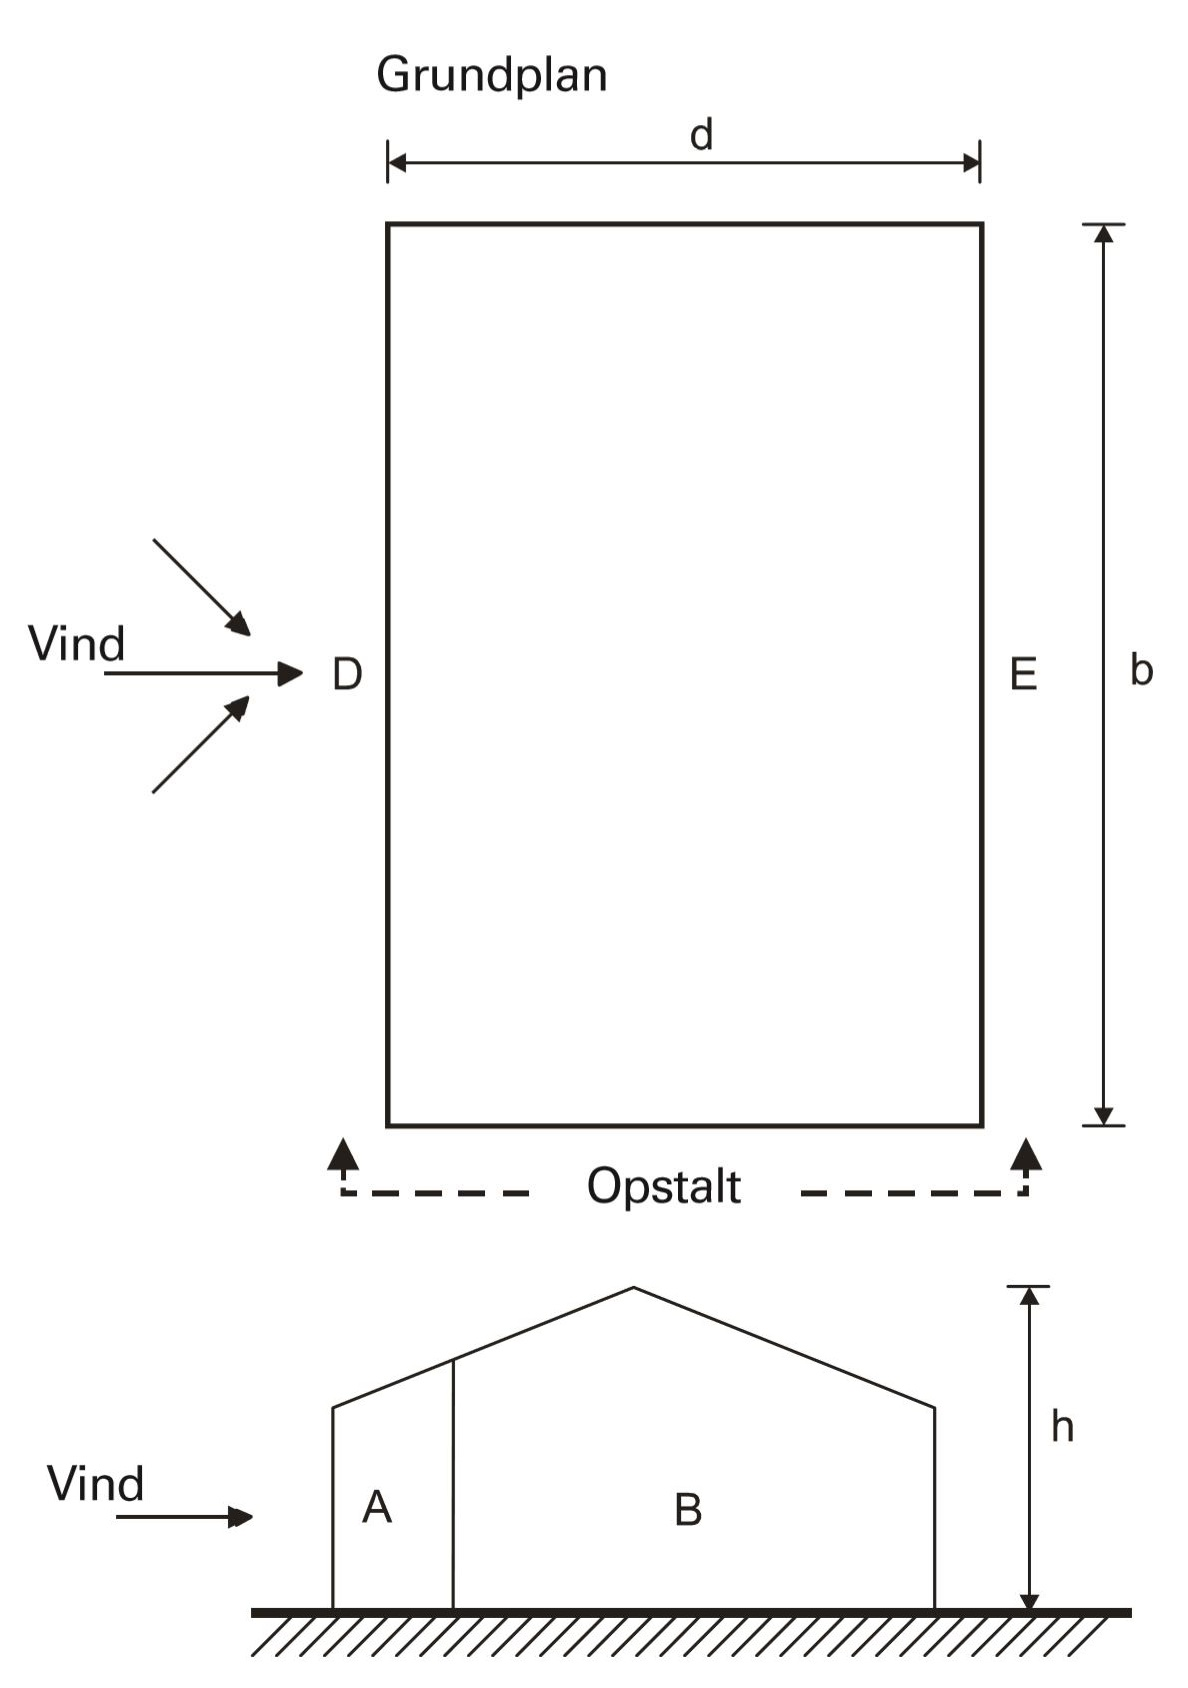
\includegraphics[width=0.60\textwidth]{billeder/Vindlast1}
\caption{Sadeltag med to forskellige skråninger og dermed to hældninger.}
\label{fig:SF1}
\end{figure}



\subsubsection{Vindlast på taget}

\begin{figure}[H] 
\centering
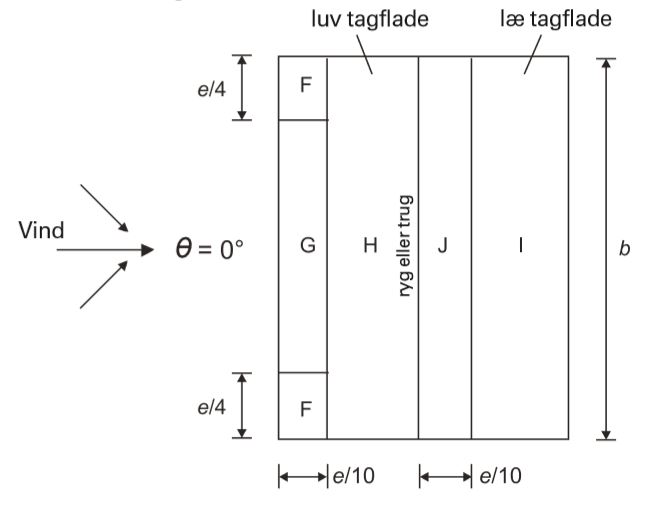
\includegraphics[width=0.60\textwidth]{billeder/Vindlast3}
\caption{Sadeltag med to forskellige skråninger og dermed to hældninger.}
\label{fig:SF1}
\end{figure}





















\section{Snelast}
Ved beregning af belastninger på en given konstruktion, så skal man også tage stilling til snelasten. Snelasten på tilbygningen regnes med formlen for vedvarende/midlertidig dimensioneringstilfælde:

$s = \mu_i \cdot C_e  \cdot  C_t \cdot s_k$

hvor

\begin{itemize}
\item $\mu_i$ = formfaktor.
\item $C_e$ = eksponeringsfaktor.
\item $C_t$ = termisk faktor
\item $s_k = karakteristisk snelast på jorden$
\end{itemize}


\subsection{Formfaktor}
Formfaktoren afhænger af tagtype og dens hældning. Tilbygningen er beklædt med et saddeltag med følgende vinkler som kan ses på figur 1: 

\begin{figure}[H] 
\centering
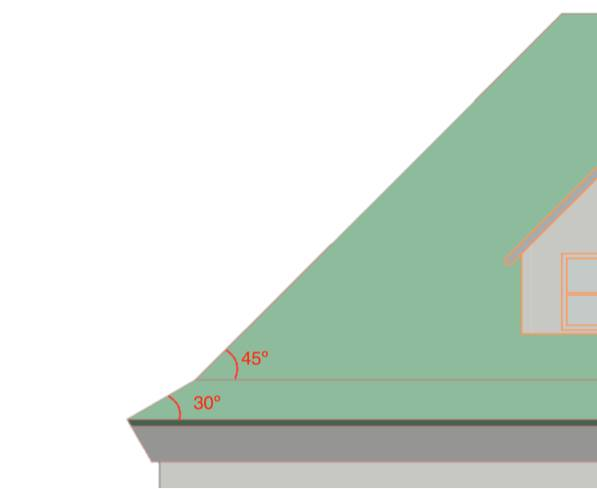
\includegraphics[width=0.60\textwidth]{billeder/SnelastFigur1}
\caption{Sadeltag med to forskellige skråninger og dermed to hældninger.}
\label{fig:SF1}
\end{figure}

Formfaktoren inddeles i tre dele; den ene med hældning på 30º, den anden med en hældning på 45º og til sidst det flade tagstykke. Form faktoren for den skrå hældning med 30º er 0,8. For den skrå hældning med 45º er værdien 0,4 og for det flade tag er værdien 0,8. 

\subsection{Eksponeringsfaktor}
Denne faktor er afhængig af omgivelserne omkring tilbygningen, men også dimensionerne på bygningen spiller en rolle. Deraf kommer formlen:

$C_e = C_{top} \cdot  C_s$

Topografien inddeles i enten vindblæst, normal eller afskærmet, alt efter hvor blottet konstruktionen. Da tilbygningen delvis er afskærmet og delvis vindblæst, så vælges der her den maksimale mulige værdi for topografien for at tage stilling til den værst mulige belastning der måtte forekomme. Værdien for topografien sættes dermed til 1,25.

Faktoren for dimensionen af konstruktionen sættes til at være lig med 1,0. Dette skyldes at den opfylder følgende sætning: $2h > l_1$, hvor $h$ svarer til højden af konstruktionen og $l_1$ svarer til den længste side af bygningen.

Eksponeringsfaktor kommer da til at få værdien på 1,25.

\subsection{Termisk faktor}
Følgende faktor bruges som en reduktionsfaktor i det tilfælde hvor der er høj varmeoverførsel såsom et drivhus med glastag. Under normale omstændigheder sættes den termisk faktor til at være 1,0.

\subsection{Karakteristisk terrænværdi}
Denne værdi sættes til at være lig med $\SI{1}{ kN/m^2}$ i Danmark

\subsection{Beregning af snelast}
De fundende faktor og variabler kan nu bruges til at finde snelasten på tilbygningen. Værdierne kan findes i tabellen forneden:

\begin{table}[H]
\centering
\begin{tabular}{|l|c|c|}
\hline
\textbf{Beskrivelse}       & \textbf{Symbol} & \textbf{Værdi}                                                                                    \\ \hline
Formfaktor                 & $\mu_i$               & \begin{tabular}[c]{@{}c@{}}0,8 (hældning 30º)\\ 0,4 (hældning 45º)\\ 0,8 (fladt tag)\end{tabular} \\ \hline
Eksponeringsfaktor         & $C_e$               & 1,25                                                                                              \\ \hline
- Topografi                & $C_{top}$               & 1,25                                                                                              \\ \hline
- Faktor for dimension     & $C_s$               & 1,0                                                                                               \\ \hline
Termisk faktor             & $C_t$               & 1,0                                                                                                 \\ \hline
Karakteristisk terrænværdi & $s_k$               & $\SI{1,0}{kN/m^2}$                                                                                              \\ \hline
\end{tabular}
\caption{Oversigt over de fundende værdier til beregning af snelast}
\label{tab:SLT1}
\end{table}


De forskellige værdier bruges til at beregne snelasten og følgende resultater kan ses i tabel \ref{tab:SLT2} Linjelasten er også beregnet over det stykke som sneen påvirket med.

\begin{table}[H]
\centering
\begin{tabular}{|l|c|c|c|}
\hline
\textbf{Tagdel}            & \textbf{Last} & \textbf{Længde} & \textbf{Linjelast} \\ \hline
Skrå del (hældning på 30º) & $\SI{1,0}{kN/m^2}$                      & 0,86 m $\cdot$ 2              & $\SI{1,73}{kN/m^2}$                                                                                                               \\ \hline
Skrå del (hældning på 45º) & $\SI{0,5}{kN/m^2}$                                     & 2,28 m $\cdot$ 2               & $\SI{4,55}{kN/m^2}$                                                                                                              \\ \hline
Fladt tag                  & $\SI{1,0}{kN/m^2}$                     &  5 m               & $\SI{5,0}{kN/m^2}$                                                                                                               \\ \hline
\end{tabular}
\caption{Oversigt over de forskellige laster for de forskellige dele som taget er blevet inddelt i.}
\label{tab:SLT2}
\end{table}


\subsection{Snelast fra sneophobning}
For bygningskonstruktioner som både udsættes for sne og vind, så regnes der med en ekstra lastarrangement. Vindsiden på sadeltaget vil have en formfaktor på nul, mens læsiden vil have en formfaktor afhængig af hældningen. Men inden der tages hensyn til den ekstra lastarrangement, så skal følgende sætninger være opfyldte:





\begin{enumerate}
\item bygningens orientering vender mod den østlige retning (fra NNØ til SØ)
\item facadehøjden i vindsiden er højst 10 m.
\item bygningens længde på tværs af vindsiden er to gange større end bygningens kiphøje
\item bygningens dybde er større end bygningens kiphøjde
\item terrænnet i vindsiden er åben i en afstand på 400 m.
\end{enumerate}

Da tilbygningen til Strøybergs Palæ opfylder alle betingelserne, så skal der regnes med ekstra last.  Igen ses der på figur 1, da de forskellige formfaktor som bruges til at udregne snelasten afhænger af hældningen på taget. For et tag med hældningen fra 15º til 30º beregnes formfaktoren til at være lig med 1,2. Derimod beregnes formfaktoren til at være 0,60 for taget med hældningen 45º. 

Til beregning af den ekstra snelast bruges den samme formel som tidligere anvendt i starten af kapitlet. Igen bruges denne formel til at beregne den ekstra snelast, formfaktoren er blot ændret:

$s = \mu_i \cdot C_e  \cdot  C_t \cdot s_k$

Resultatet kan ses i tabel \ref{tab:SLT3} hvor linjelasten også er skrevet ind.

\begin{table}[H]
\centering
\begin{tabular}{|l|c|c|c|}
\hline
\textbf{Tagdel}            & \textbf{Last} & \textbf{Længde} & \textbf{Linjelast} \\ \hline
Skrå del (hældning på 30º) & $\SI{0,75}{kN/m^2}$                      & 0,86 m $\cdot$ 2              & $\SI{2,59}{kN/m^2}$                                                                                                               \\ \hline
Skrå del (hældning på 45º) & $\SI{0,5}{kN/m^2}$                                     & 2,28 m $\cdot$ 2               & $\SI{6,82}{kN/m^2}$                                                                                                              \\ \hline
\end{tabular}
\caption{Oversigt over de ekstra snelaster der fremkommer ved låsiden ved vindblæst.}
\label{tab:SLT3}
\end{table}














